\documentclass[11pt,a4paper]{article}
\usepackage[margin=18mm]{geometry}
\usepackage{amsmath,amssymb,mathtools}
\usepackage{booktabs,array,enumitem}
\usepackage[dvipsnames]{xcolor}
\usepackage{graphicx,listings,tikz,float,needspace}
\usetikzlibrary{arrows.meta,positioning}
\usepackage[most]{tcolorbox}
\usepackage{hyperref}
\hypersetup{colorlinks=true,urlcolor=MidnightBlue,linkcolor=MidnightBlue}
\setlength{\parindent}{0pt}\setlength{\parskip}{4pt}
\newcommand{\course}{PHY4605 Computational Methods in Physics}
\newcommand{\units}[1]{\,\mathrm{#1}}
\newtcolorbox{keybox}{colback=RoyalBlue!5,colframe=RoyalBlue!65!black,boxrule=.7pt,arc=2mm}
\newtcolorbox{checkbox}{colback=ForestGreen!5,colframe=ForestGreen!55!black,boxrule=.7pt,arc=2mm}
\newtcolorbox{aibox}{colback=BurntOrange!7,colframe=BurntOrange!80!black,boxrule=.7pt,arc=2mm}
\lstdefinestyle{matlabstyle}{language=Matlab,basicstyle=\ttfamily\footnotesize,keywordstyle=\color{RoyalBlue!75!black},commentstyle=\color{ForestGreen!55!black},stringstyle=\color{BurntOrange!80!black},numbers=left,numberstyle=\scriptsize\color{black!50},numbersep=5pt,frame=single,rulecolor=\color{RoyalBlue!25},backgroundcolor=\color{RoyalBlue!3},showstringspaces=false,columns=fullflexible,keepspaces=true,breaklines=true}
\begin{document}
{\large\textsc{\course}}\\[-2pt]
{\small Learning Note \textbar\ Week 10}\par\vspace{4pt}
{\LARGE\bfseries Random Sampling and Monte Carlo:\\From One Random Path to Reliable Evidence}\par\vspace{3pt}
\textit{Use repeated random trials to describe physical variability, test reproducibility, and see how sample size affects a Monte Carlo estimate.}

\begin{keybox}\textbf{Physical question.} A small particle receives random left-or-right kicks. One path is unpredictable, but if we simulate many particles under the same rule, what stable pattern can we extract from their final positions?\end{keybox}

\section*{Core learning outcomes}
\begin{enumerate}[nosep,leftmargin=5mm]
\item explain what one random trial represents physically and reproduce a supplied random-sampling scaffold;
\item calculate and interpret the mean and spread of repeated outcomes; and
\item compare several sample sizes, use a fixed random seed when required, and validate the result against the physical model.
\end{enumerate}

\section*{1. A random model still needs a physical rule}
The lecture model is a one-dimensional symmetric random walk. A particle starts at
\[
x_0=0\units{mm}.
\]
Every second it moves exactly one step of length
\[
a=1\units{mm},
\]
either to the right or to the left with equal probability. After $N=100$ steps, the particle has one final position. We do not know that position in advance because the sequence of directions is random.

The randomness is bounded by a precise model: every step has the same magnitude, the two directions are equally likely, and successive steps are treated as independent. If any of those assumptions changes, the expected distribution of final positions also changes.

\begin{checkbox}\textbf{Prediction checkpoint.} The model has no preferred direction. Across many independent particles, the average final position should therefore be near $0\units{mm}$. Individual particles should still finish at many different positions.\end{checkbox}

\section*{2. What exactly is one Monte Carlo trial?}
For this model, \textbf{one trial is one complete 100-step path}. One trial contains many random draws, but it produces one main repeated outcome: the final position after 100 steps.

Repeating the Monte Carlo experiment means simulating many independent 100-step paths under the same physical assumptions. The number of repeated paths is the Monte Carlo sample size $M$.

Keep these two counts separate:

\begin{center}\small
\begin{tabular}{p{.25\linewidth}p{.27\linewidth}p{.37\linewidth}}
\toprule
Quantity & Week 10 value & Meaning\\
\midrule
$N$ & 100 steps/trial & Physical duration of one random path\\
$a$ & $1\units{mm}$/step & Physical step length\\
$M$ & 100, 1000, or 10000 trials & Number of independent paths used for the estimate\\
\bottomrule
\end{tabular}
\end{center}

Increasing $N$ changes the physical walk itself. Increasing $M$ gives more repeated evidence about the same 100-step model.

\section*{3. Turn random draws into physical steps}
The computational rule is simple:

\begin{enumerate}[nosep,leftmargin=7mm]
\item choose $N$, $a$, $M$, and a random seed when an exact rerun is required;
\item generate one random number for every step of every trial;
\item map values below $0.5$ to $-a$ and values at least $0.5$ to $+a$;
\item cumulatively sum the steps to obtain trajectories;
\item extract the final position from each trial;
\item calculate the mean and spread of the final positions;
\item compare summaries for several values of $M$; and
\item validate the numerical evidence against symmetry and the known step rule.
\end{enumerate}

This is the same course reasoning chain used in earlier weeks: physical model $\rightarrow$ algorithm $\rightarrow$ code $\rightarrow$ numerical evidence $\rightarrow$ validation $\rightarrow$ interpretation.

\Needspace{21\baselineskip}
\section*{4. MATLAB random-sampling scaffold}
Base MATLAB provides the random numbers. The Week 10 learning target is reading and modifying the scaffold, not deriving a random-number generator.

\begin{lstlisting}[style=matlabstyle]
n_steps = 100;
step_length_mm = 1;
maximum_trials = 10000;

rng(4605,'twister')
u = rand(n_steps,maximum_trials);
direction = 2*(u >= 0.5)-1;
step_mm = step_length_mm*direction;

trajectory_mm = cumsum(step_mm,1);
final_position_mm = trajectory_mm(end,:);
\end{lstlisting}

The expression \texttt{u >= 0.5} produces logical values. Multiplying by 2 and subtracting 1 converts them to $-1$ or $+1$. Multiplying by \texttt{step\_length\_mm} attaches the physical step scale.

\begin{aibox}\textbf{Do not confuse the seed with a physical parameter.} The seed chooses a reproducible random-number sequence. It does not represent time, position, temperature, or a property of the particle. Changing the seed should change finite-sample details while preserving the statistical behaviour of a correct model.\end{aibox}

\section*{5. One trajectory is one possible history}
The first simulated path below is produced with the locked seed. Another valid seed can produce a very different-looking path.

\begin{figure}[H]
\centering
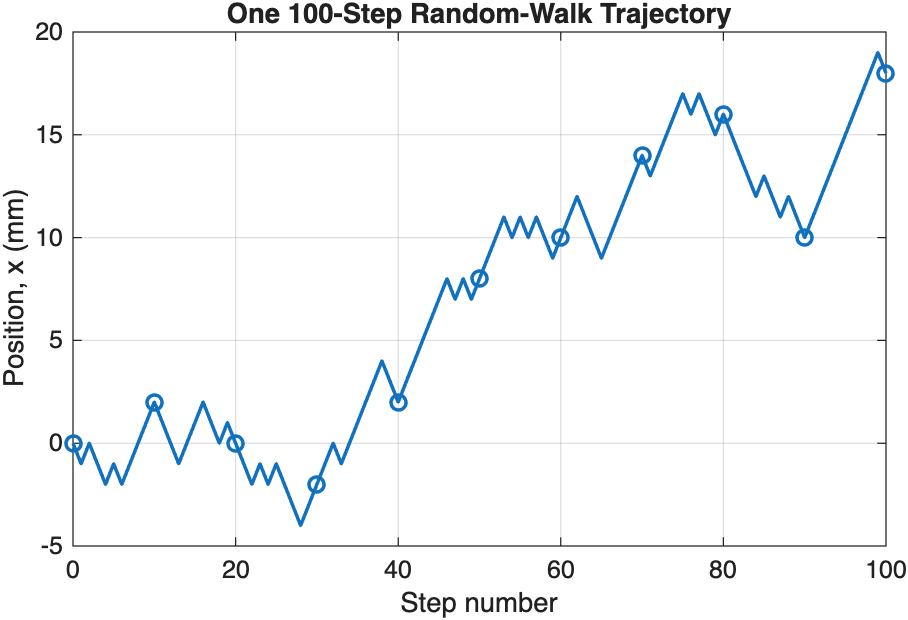
\includegraphics[width=.76\linewidth]{assets/week10_random_walk_trajectory.png}
\caption{One 100-step random-walk trajectory. The path is physically possible under the model, but it is not the unique or ``correct'' path.}
\end{figure}

A trajectory is useful for connecting the code to motion, but one trajectory cannot tell us the long-run mean or spread. Those require repeated trials.

\section*{6. Repeated trials produce a distribution}
With $M=10000$ independent paths, the locked simulation gives a distribution of final positions.

\begin{figure}[H]
\centering
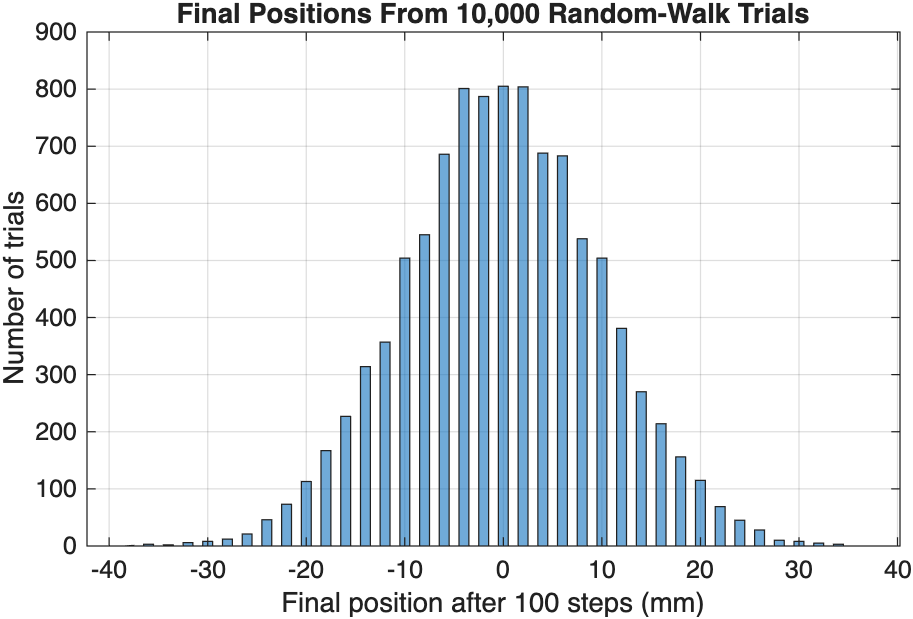
\includegraphics[width=.73\linewidth]{assets/week10_random_walk_histogram.png}
\caption{Final positions after 100 steps for 10000 repeated trials. The distribution is centred near zero but individual final positions vary widely.}
\end{figure}

For these 10000 trials,
\[
\overline{x}_{\mathrm{final}}=-0.128\units{mm},
\qquad
s_{\mathrm{final}}=9.9423\units{mm}.
\]

The \textbf{mean} describes the centre of the repeated outcomes. The \textbf{spread} describes how widely individual outcomes vary around that centre. A mean near zero does not mean every particle finishes at zero.

\begin{checkbox}\textbf{Core interpretation check.} If the final-position mean is close to $0\units{mm}$ but the spread is about $10\units{mm}$, the two results are not contradictory. Symmetry controls the centre; accumulated random steps create the variability.\end{checkbox}

\section*{7. Sample size changes the estimate, not the physical walk}
Use the first 100, 1000, and 10000 trials from the same reproducible simulation:

\begin{center}\small
\begin{tabular}{rrr}
\toprule
Repeated trials $M$ & Mean final position (mm) & Spread (mm)\\
\midrule
100 & 0.040 & 10.6320\\
1000 & 0.066 & 9.8122\\
10000 & -0.128 & 9.9423\\
\bottomrule
\end{tabular}
\end{center}

The mean does not move monotonically toward zero: $0.040$, $0.066$, then $-0.128\units{mm}$. Random convergence can fluctuate. What matters is that all three values are small compared with the roughly $10\units{mm}$ spread and are consistent with a centre near zero.

\begin{figure}[H]
\centering
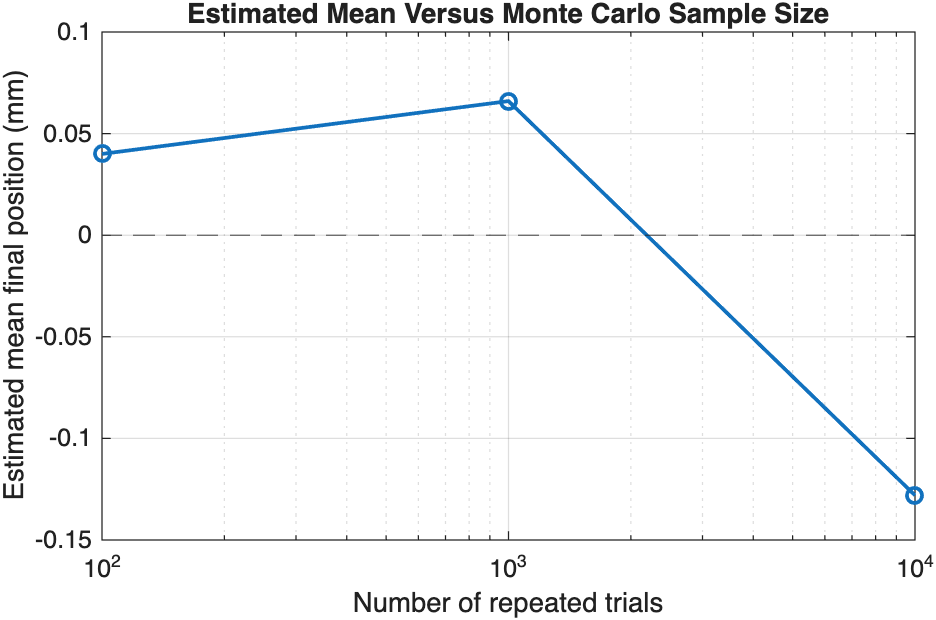
\includegraphics[width=.71\linewidth]{assets/week10_random_walk_sample_size.png}
\caption{The finite-sample mean changes as more trials are included. More trials generally stabilise an estimate, but one random sequence need not approach the reference monotonically.}
\end{figure}

The spread stays near $10\units{mm}$ for all three sample sizes because the underlying 100-step physical process has not changed. More Monte Carlo trials improve our evidence about the distribution; they do not make individual random walks less variable.

\section*{8. Validate with the model, not with appearance alone}
Two Core checks follow directly from the physical rule.

\textbf{Symmetry check.} Equal left/right probabilities imply a long-run mean near $0\units{mm}$. The locked mean $-0.128\units{mm}$ is small compared with the width of the distribution.

\textbf{Step-rule check.} After exactly 100 steps of $\pm1\units{mm}$, every final position must be an even integer number of millimetres. A result such as $7.3\units{mm}$ would violate the model even if it appeared inside a plausible-looking histogram.

\begin{aibox}\textbf{A reproducible wrong model is still wrong.} Resetting a seed can reproduce a coding defect perfectly. Always pair reproducibility with a physical or numerical validation check.\end{aibox}

\section*{9. Worked reasoning chain}
\begin{center}\small
\begin{tabular}{p{.25\linewidth}p{.67\linewidth}}
\toprule
Step & Week 10 evidence\\
\midrule
Physical model & symmetric 1D walk, $100$ steps of $\pm1\units{mm}$\\
Scale and units & position and step length in mm; trial count is dimensionless\\
Algorithm & random draw $\rightarrow$ direction $\rightarrow$ cumulative position $\rightarrow$ repeat\\
Code & supplied \texttt{rng}, \texttt{rand}, logical mapping, \texttt{cumsum}\\
Variability & distribution of final positions, mean, and spread\\
Validation & symmetry near zero plus even-integer final-position rule\\
Interpretation & more trials stabilise estimates without removing physical randomness\\
\bottomrule
\end{tabular}
\end{center}

In an assessment, syntax may be supplied. You still need to define one trial, explain what repeated outcomes mean, keep physical units, distinguish mean from spread, and justify a validation check.

\section*{Working exposure: standard error and random-walk scaling}
A supplied standard-error estimate for the mean is
\[
\mathrm{SE}(\overline{x})\approx\frac{s}{\sqrt{M}}.
\]
For the locked simulation, the supplied values are about $1.063$, $0.310$, and $0.099\units{mm}$ for $M=100$, 1000, and 10000. Standard error describes precision of the \emph{estimated mean}, not particle spread.

For the ideal symmetric walk, the supplied final-position scaling is
\[
s_x\sim a\sqrt{N}.
\]
With $a=1\units{mm}$ and $N=100$, this gives $10\units{mm}$; the simulated $9.9423\units{mm}$ is close. Interpreting the scaling is Working exposure; deriving it is not required.

\section*{Optional stretch}
Distribution derivations, statistical mechanics, variance reduction, MCMC diagnostics, and formal convergence theory are outside the Week 10 Core route.

\section*{Three takeaways}
\begin{enumerate}[nosep,leftmargin=7mm]
\item One trial needs a physical meaning; here it is one complete 100-step path.
\item Mean describes the centre; spread describes variability of individual outcomes.
\item A fixed seed supports reproducibility; sample-size and physical checks support trustworthiness.
\end{enumerate}

\begin{keybox}\textbf{Preparation for the practical.} Be ready to identify one random trial, trace a supplied random-sampling scaffold, interpret a histogram or summary table, compare sample sizes, use a fixed seed when needed, and validate the Monte Carlo result against independent physical evidence.\end{keybox}

\end{document}
